\documentclass[11pt]{article}

%% PACKAGES
\usepackage{graphicx}
\usepackage[printonlyused]{acronym}
\usepackage{float}
\usepackage{tabularx}
\usepackage[colorlinks=false]{hyperref}
\usepackage{caption}
\usepackage[margin=1.0in]{geometry}
\usepackage{tocloft}

\makeatletter
\g@addto@macro\normalsize{%
  \setlength\abovedisplayskip{0.25pt}
  \setlength\belowdisplayskip{0.25pt}
  \setlength\abovedisplayshortskip{0.25pt}
  \setlength\belowdisplayshortskip{0.25pt}
}
\makeatother

\setlength{\parskip}{\baselineskip}

%% GRAPHICS PATH
\graphicspath{{../../../shared_latex_inputs/images}{../../../shared_latex_inputs/graphs}}

\title{\Huge EMTG Tutorial: Introduction and Setup}
\vspace{0.5cm}
\author
{
	Tim Sullivan \thanks{Aerospace Engineer, The Aerospace Corporation}
}
\vspace{0.5cm}

\newcommand{\listofknownissuesname}{\Large List of Known Issues}
\newlistof{knownissues}{mcf}{\listofknownissuesname}

\newcommand{\knownissue}[3]
{
	\refstepcounter{knownissues}
	\par\noindent\textbf{\hyperref[#2_b]{\theknownissues\quad #1}}\label{#2_h}
	\textbf{\hfill\pageref{#2_b}}
	#3
}

\newcommand{\knownissuelabel}[2]
{
	 \phantomsection
  	\hyperref[#2_h]{#1}\def\@currentlabel{\unexpanded{#1}}\label{#2_b}
}

\begin{document}

\begin{titlepage}
\maketitle
\thispagestyle{empty}
\begin{table}[H]
	\centering
	\begin{tabularx}{\textwidth}{|l|l|X|}
		\hline
		\textbf{Revision Date} & \textbf{Author} & \textbf{Description of Change} \\
		\hline
		\date{December 2, 2022} & Tim Sullivan & Initial revision.\\
		\hline
		\date{June 30, 2023} & Joseph Hauerstein & Conversion to \LaTeX.\\ 
		\hline
		\date{August 4, 2023} & Joseph Hauerstein & Addition of Known Issues section.\\ 
		\hline
	\end{tabularx}
\end{table}
\end{titlepage}

\newpage
\tableofcontents
\thispagestyle{empty}
\newpage

\listofknownissues
\thispagestyle{empty}


\newpage
\clearpage
\setcounter{page}{1}



%\section*{List of Acronyms}
\begin{acronym}
%To define the acronym and include it in the list of acronyms: \acro{acronym}{definition}
%To define the acronym and exclude it from the list of acronyms:  \acro{acronym}{definition}
%
%\ac{acronym} Expand and identify the acronym the first time; use only the acronym thereafter
%\acf{acronym} Use the full name of the acronym.
%\acs{acronym} Use the acronym, even before the first corresponding \ac command
%\acl{acronym}  Expand the acronym without using the acronym itself.
%
%

\acro{TCM}{trajectory correction maneuver}
\acro{ACO}{Ant Colony Optimization}
\acro{AD}{Automatic Differentiation}
\acro{ADL}{Architecture Design Laboratory}
\acro{ADM}{asteroid departure maneuver}
\acro{AEI}{atmospheric entry interface}
\acro{AES}{Advanced Exploration Systems}
\acro{AGA}{aerogravity assist}
\acro{ALARA}{As Low As Reasonably Achievable}
\acro{API}{application programming interface}
\acro{BB}{branch and bound}
\acro{BVP}{Boundary Value Problem}
\acro{CATO}{Computer Algorithm for Trajectory Optimization}
\acro{CL}{confidence level}
\acro{CONOPS}{concept of operations}
\acro{COV}{Calculus of Variations}
\acro{D/AV}{Descent/Ascent Vehicle}
\acro{DE}{Differential Evolution}
\acro{RLA}{Right Ascension of Launch Asymptote}
\acro{DLA}{Declination of Launch Asymptote}
\acro{DPTRAJ/ODP}{Double Precision Trajectory and Orbit Determination Program}
\acro{DSH}{Deep Space Habitat}
\acro{DSN}{Deep Space Network}
\acro{DSMPGA}{Dynamic-Size Multiple Population Genetic Algorithm}
\acro{EB}{Evolutionary Branching}
\acro{ECLSS}{environmental control and life support system}
\acro{EGA}{Earth gravity assist}
\acro{ELV}{expendable launch vehicle}
\acro{EMME}{Earth to Mars, Mars to Earth}
\acro{EMMVE}{Earth to Mars, Mars to Venus to Earth}
\acro{EMTG}{Evolutionary Mission Trajectory Generator}
\acro{EVMME}{Earth to Venus to Mars, Mars to Earth}
\acro{EVMMVE}{Earth to Venus to Mars, Mars to Venus to Earth}
\acro{ERRV}{Earth Return Re-entry Vehicle}
\acro{FISO}{Future In-Space Operations}
\acro{FMT}{Fast Mars Transfer}
\acro{GASP}{Gravity Assist Space Pruning}
\acro{GCR}{galactic cosmic radiation}
\acro{GRASP}{Greedy Randomized Adaptive Search Procedure}
\acro{GSFC}{Goddard Space Flight Center}
\acro{GTOC}{Global Trajectory Optimization Competition}
\acro{GTOP}{Global Trajectory Optimization Problem}
\acro{HAT}{Human Architecture Team}
\acro{HGGA}{Hidden Genes Genetic Algorithm}
\acro{IMLEO}{Initial Mass in \acl{LEO}}
\acro{IPOPT}{Interior Point OPTimizer}
\acro{ISS}{International Space Station}
\acro{JHUAPL}{Johns Hopkins University Applied Physics Laboratory}
\acro{JSC}{Johnson Space Center}
\acro{KKT}{Karush-Kuhn-Tucker}
\acro{LEO}{Low Earth Orbit}
\acro{LRTS}{lazy race tree search}
\acro{MAT}{Mars Architecture Team}
\acro{MONTE}{Mission analysis, Operations, and Navigation Toolkit Environment}
\acro{MCTS}{Monte Carlo tree search}
\acro{MGA}{Multiple Gravity Assist}
\acro{MIRAGE}{Multiple Interferometric Ranging Analysis using GPS Ensemble}
\acro{MOGA}{Multi-Objective Genetic Algorithm}
\acro{MOSES}{Multiple Orbit Satellite Encounter Software}
\acro{MPI}{message passing interface}
\acro{MPLM}{Multi-Purpose Logistics Module}
\acro{MSFC}{Marshall Space Flight Center}
\acro{NELLS}{NASA Exhaustive Lambert Lattice Search}
\acro{NMDB}{Navigation and Mission Design Branch}
\acro{NSGA}{Non-Dominated Sorting Genetic Algorithm}
\acro{NSGA-II}{Non-Dominated Sorting Genetic Algorithm II}
\acro{NHATS}{Near-Earth Object Human Space Flight Accessible Targets Study}
\acro{NTP}{Nuclear Thermal Propulsion}
\acro{OD}{orbit determination}
\acro{OOS}{On-Orbit Staging}
\acro{PCC}{Pork Chop Contour}
\acro{PEL}{permissible exposure limits}
\acro{PLATO}{PLAnetary Trajectory Optimization}
\acro{REID}{risk of exposure-induced death}
\acro{RTBP}{Restricted Three Body Problem}
\acro{SA}{Simulated Annealing}
\acro{SLS}{Space Launch System}
\acro{SNOPT}{Sparse Nonlinear OPTimizer}
\acro{SOI}{sphere of influence}
\acro{SPE}{solar particle events}
\acro{SQP}{sequential quadratic programming}
\acro{SRAG}{Space Radiation Analysis Group}
\acro{TEI}{Trans-Earth Injection}
\acro{TIM}{technical interchange meeting}
\acro{TOF}{time of flight}
\acro{TPBVP}{Two Point Boundary Value Problem}
\acro{TMI}{Trans-Mars Injection}
\acro{VARITOP}{Variational calculus Trajectory Optimization Program}
\acro{VGA}{Venus gravity assist}
\acro{VILM}{v-infinity leveraging maneuver}
\acro{MOI}{Mar Orbit Injection}
\acro{PCM}{Pressurized Cargo Module}
\acro{STS}{Space Transportation System}
\acro{EDS}{Earth Departure Stage}
\acro{NEO}{near-Earth asteroid}
\acro{IDC}{Integrated Design Center}
\acro{SEP}{solar-electric propulsion}
\acro{SRP}{solar radiation pressure}
\acro{NEP}{nuclear-electric propulsion}
\acro{REP}{radioisotope-electric propulsion}
\acro{DRM}{Design Reference Missions}

\acro{ASCII}{American Standard Code for Information Interchange}
\acro{AU}{Astronomical Unit}
\acro{BWG}{Beam Waveguides}
\acro{CCB}{Configuration Control Board}
\acro{CMO}{Configuration Management Office}
\acro{CODATA}{Committee on Data for Science and Technology}
\acro{DEEVE}{Dynamically Equivalent Equal Volume Ellipsoid}
\acro{DRA}{Design Reference Asteroid}
\acro{EME2000}{Earth Centered, Earth Mean Equator and Equinox of J2000 (Coordinate Frame)}
\acro{EOP}{Earth Orientation Parameters}
\acro{ET}{Ephemeris Time}
\acro{FDS}{Flight Dynamics System}
\acro{FTP}{File Transfer Protocol}
\acro{GSFC}{Goddard Space Flight Center}
\acro{PI}{Principal Investigator}
\acro{HEF}{High Efficiency}
\acro{IAG}{International Association of Geodesy}
\acro{IAU}{International Astronomical Union}
\acro{IERS}{International Earth Rotation and Reference Systems Service}
\acro{ICRF}{International Celestial Reference Frame}
\acro{ITRF}{International Terrestrial Reference System}
\acro{IOM}{Interoffice Memorandum}
\acro{JD}{Julian Date}
\acro{JPL}{Jet Propulsion Laboratory}
\acro{LM}{Lockheed Martin}
%\acro{LP150Q}{}
%\acros{LP100K}{}
\acro{MAVEN}{Mars Atmosphere and Volatile EvolutioN}
\acro{MJD}{Modified Julian Date}
\acro{MOID}{Minimum Orbit Intersection Distance}
\acro{MPC}{Minor Planet Center}
\acro{NASA}{National Aeronautics and Space Administration}
\acro{NDOSL}{\ac{NASA} Directory of Station Locations}
\acro{NEA}{near-Earth asteroid}
\acro{NEO}{near-Earth object}
\acro{NIO}{Nav IO}
\acro{OSIRIS-REx}{Origins, Spectral Interpretation, Resource Identification, and Security-Regolith Explorer}
\acro{PHA}{Potentially Hazardous Asteroid}
\acro{PHO}{Potentially Hazardous Object}
\acro{SBDB}{Small-Body Database}
\acro{SI}{International System of Units}
\acro{SPICE}{Spacecraft Planet Instrument Camera-matrix Events}
\acro{SPK}{SPICE Kernel}
\acro{SRC}{Sample Return Capsule}
\acro{SSD}{Solar System Dynamics}
\acro{AGI}{Analytical Graphics, Inc.}
\acro{STK}{Systems Tool Kit}
\acro{TAI}{International Atomic Time}
\acro{TBD}{To Be Determined}
\acro{TBR}{To Be Reviewed}
\acro{TCB}{Barycentric Coordinate Time}
\acro{TDB}{Temps Dynamiques Barycentrique, Barycentric Dynamical Time}
\acro{TDT}{Terrestrial Dynamical Time}
\acro{TT}{Terrestrial Time}
\acro{URL}{Uniform Resource Locator}
\acro{UT}{Universal Time}
\acro{UT1}{Universal Time Corrected for Polar Motion}
\acro{UTC}{Coordinated Universal Time}
\acro{USNO}{U. S. Naval Observatory}
\acro{YORP}{Yarkovsky-O'Keefe-Radzievskii-Paddack}

\acro{NLP}{nonlinear program}
\acro{MBH}{monotonic basin hopping}
\acro{MBH-C}{monotonic basin hopping with Cauchy hops}
\acro{FBS}{forward-backward shooting}
\acro{MGALT}{Multiple Gravity Assist with Low-Thrust}
\acro{MGALTS}{Multiple Gravity Assist with Low-Thrust using the Sundman transformation}
\acro{MGA-1DSM}{Multiple Gravity Assist with One Deep Space Maneuver}
\acro{MGAnDSMs}{Multiple Gravity Assist with $n$ Deep-Space Maneuvers using Shooting}
\acro{PSFB}{Parallel Shooting with Finite-Burn}
\acro{PSBI}{Parallel Shooting with Bounded Impulses}
\acro{FBLT}{Finite-Burn Low-Thrust}
\acro{FBLTS}{Finite-Burn Low-Thrust using the Sundman transformation}
\acro{ESA}{European Space Agency}
\acro{ACT}{Advanced Concepts Team}
\acro{IRAD}{independent research and development}
\acro{Isp}[$\text{I}_{sp}$]{specific impulse}
\acro{GA}{genetic algorithm}
\acro{GALLOP}{ Gravity Assisted Low-thrust Local Optimization Program}
\acro{MALTO}{Mission Analysis Low-Thrust Optimization}
\acro{PaGMO}{Parallel Global Multiobjective Optimizer}
\acro{FRA}{feasible region analysis}
\acro{CP}{conditional penalty}
\acro{HOC}{hybrid optimal control}
\acro{HOCP}{hybrid optimal control problem}
\acro{PSO}{particle swarm optimization}
\acro{SEPTOP}{Solar Electric Propulsion Trajectory Optimization Program}
\acro{STOUR}{Satellite Tour Design Program}
\acro{STOUR-LTGA}{Satellite Tour Design Program - Low Thrust, Gravity Assist}
\acro{PaGMO}{Parallel Global Multiobjective Optimizer}
\acro{SDC}{static/dynamic control}
\acro{DDP}{Differential Dynamic Programming}
\acro{HDDP}{Hybrid Differential Dynamic Programming}
\acro{ACT}{Advanced Concepts Team}
\acro{GMAT}{General Mission Analysis Toolkit}
\acro{BOL}{beginning of life}
\acro{EOL}{end of life}
\acro{KSC}{Kennedy Space Center}
\acro{VSI}{variable \ac{Isp}}
\acro{RTG}{radioisotope thermal generator}
\acro{ASRG}{advanced Stirling radiosotope generator}
\acro{ARRM}{Asteroid Robotic Redirect Mission}
\acro{AATS}{Alternative Architecture Trade Study}
\acro{PPU}{power processing unit}
\acro{STM}{state transition matrix}
\acro{MTM}{maneuver transition matrix}
\acro{BCI}{body-centered inertial}
\acro{BCF}{body-centered fixed}
\acro{UTTR}{Utah Test and Training Range}
\acro{EPV}{equatorial projection of $\mathbf{v}_\infty$}
\acro{KBO}{Kuiper belt object}
\acro{DSM}{deep-space maneuver}
\acro{BPT}{body-probe-thrust}
\acro{4PL}{four parameter logistic}
\acro{BCF}{body-centered fixed}

\acro{SPT}{Sun-probe-thrust}
\acro{PIRATE}{PVDrive Interface and Robust Astrodynamic Target Engine}
\acro{PEATSA}{Python EMTG Automated Trade Study Application}
\acro{NEXT}{NASA's Evolutionary Xenon Thruster}
\acro{TAG}{Touch and Go}
\acro{KBO}{Kuiper Belt object}

\acro{CDR}{critical design review}
\acro{PDR}{preliminary design review}
\acro{CCAFS}{Cape Canaveral Air Force Station}

\acro{MRD}{Mission Requirements Document}
\acro{EDL}{entry, descent, and landing}

\acro{Earth-GRAM}{Earth Global Reference Atmospheric Model}
\acro{POST II}{Program to Optimize Simulated Trajectories II}
\acro{MONSTER}{Monte-Carlo Operational Navigation Simulation for Trajectory Evaluation and Research}

\acro{ZSOI}{zero sphere of influence}
\end{acronym}

% --------------------------------------------------------------------------------------------------------------------------
% --------------------------------------------------------------------------------------------------------------------------


%%%%%%%%%%%%%%%%%%%%%
\section{Introduction}
\label{sec:introduction}
%%%%%%%%%%%%%%%%%%%%%

Welcome to the tutorial series on \acs{NASA}’s \ac{EMTG}. \ac{EMTG} is a tool for the design of space missions using either high-thrust chemical or low-thrust electric propulsion and, optionally, planetary flyby maneuvers. \ac{EMTG} is capable of determining both the optimal flyby sequence (using a Python-based outer loop) and also the optimal trajectory (using a nonlinear programming solver and monotonic basin hopping). \ac{EMTG} can operate at multiple levels of modeling fidelity that are suitable for trade studies, some proposals, and use as initial guesses for flight-fidelity tools. \ac{EMTG} is not an operational tool like \acs{STK}, \acs{GMAT}, or \acs{MONTE}.

\noindent \ac{EMTG} is composed of two components. The core \ac{EMTG} program is written in C++ and is driven by a text script interface. The second component is a \ac{GUI} written in Python called PyEMTG, which is used to process \ac{EMTG} input and output scripts. The two programs are independent but complementary.

%%%%%%%%%%%%%%%%%%%%%
\section{Learning Objectives}
\label{sec:learning_objectives}
%%%%%%%%%%%%%%%%%%%%%

This tutorial series provides seven introductory lessons on \ac{EMTG}. Each tutorial focuses on a different aspect of \ac{EMTG}. Each lesson builds on one or more previous lessons, so it is highly recommended that the lessons be completed in order. The lessons begin with low-fidelity chemical and low-thrust missions. Each tutorial adds additional realism and details to the initial simplistic missions, similar to the way someone might design a real-world mission.

\noindent The list of tutorials is provided below, in the order in which they should be performed. Each has an additional directory of the same name in the Tutorial\_EMTG\_Files directory with the accompanying \ac{EMTG} files the user will create during the tutorial and example \ac{EMTG} results. Each tutorial expects the user to have completed all the previous tutorials.

\begin{enumerate}
	\item \textbf{OSIRIS-REx:} Basic introduction to \ac{EMTG} chemical missions. Creates a low-fidelity, patched-conic, multi-phase mission similar to the OSIRIS-REx trajectory.
	\item \textbf{LowSIRIS-REx:} Basic introduction to \ac{EMTG} low-thrust missions. Modifies the OSIRIS-REx mission for low-thrust and introduces two transcription methods for low-thrust missions in \ac{EMTG}.
	\item \textbf{Boundary Types:} Explains how \ac{EMTG} models Journey Boundaries (departure and arrival states).
	\item \textbf{Propagation and Force Models:} Provides additional details on \ac{EMTG} “Mission Types” or transcription methods, propagation options, and perturbing forces.
	\item \textbf{Flybys:} Takes the user through the conversion of a low-fidelity patched conics mission to a high-fidelity mission with realistic flybys.
	\item \textbf{Config Files:} Explains how to configure \ac{EMTG} spacecraft and launch vehicle text configuration files to model real-world hardware and vehicles.
	\item \textbf{PEATSA:} Introduces the \ac{PEATSA}. \ac{PEATSA} allows users to explore the trade space of mission options and discover how different configurations affect the final trajectory.
\end{enumerate}

%%%%%%%%%%%%%%%%%%%%%
\section{Conventions}
\label{sec:conventions}
%%%%%%%%%%%%%%%%%%%%%

%%%%%%%%%%%%%%%%%%%%%
\subsection{Environment}
\label{sec:environment}
%%%%%%%%%%%%%%%%%%%%%

All tutorials except the \ac{PEATSA} tutorial are conducted in a Windows environment using the \ac{EMTG} Python \ac{GUI}, PyEMTG, and, occasionally, a text editor such as Notepad++. \ac{PEATSA} runs are typically conducted on a Linux multi-CPU environment, so the \ac{PEATSA} tutorial is written assuming the user has access to a Linux workstation.

\noindent \ac{EMTG} files include full paths in several locations. The \ac{EMTG} files provided were created assuming the working directory is located at \texttt{C:\textbackslash EMTG\textbackslash Tutorials\textbackslash NAME-OF-TUTORIAL}. For example, the files for the first tutorial, OSIRIS-REx, expect to be located inside \texttt{C:\textbackslash EMTG\textbackslash Tutorials\textbackslash OSIRIS-REx}. You are free to place your tutorial files wherever you want as long as you update paths appropriately.

%%%%%%%%%%%%%%%%%%%%%
\subsection{Formatting}
\label{sec:formatting}
%%%%%%%%%%%%%%%%%%%%%

Throughout the tutorials, \ac{EMTG}-specific features and naming conventions such as Universes and Journeys will be capitalized. Specific items and values the user should input in PyEMTG will be in quotations, such as "Mission Types". When discussing text in a terminal or \ac{EMTG} text file, this tutorial series will use a \texttt{monospaced font}.

%%%%%%%%%%%%%%%%%%%%%
\section{Initial EMTG Setup}
\label{sec:initial_emtg_setup}
%%%%%%%%%%%%%%%%%%%%%

These tutorials cover using \ac{EMTG} and assume that \ac{EMTG} and PyEMTG have already been installed and set up. For more information on these topics, see the files in \texttt{docs/0\_Users/build\_system} and \texttt{PyEMTG/docs}.

%%%%%%%%%%%%%%%%%%%%%
\section{Mission Directory Setup}
\label{sec:mission_directory_setup}
%%%%%%%%%%%%%%%%%%%%%

\ac{EMTG} will utilize four main directories/folders when run: the directory in which the input text file is located, Universe, Hardware, and results. For these tutorials, a working or mission directory setup for each tutorial will be created like the OSIRIS-REx directory shown in Figure \ref{fig:folder_structure}. 

\begin{figure}[H]
	\centering
	\fbox{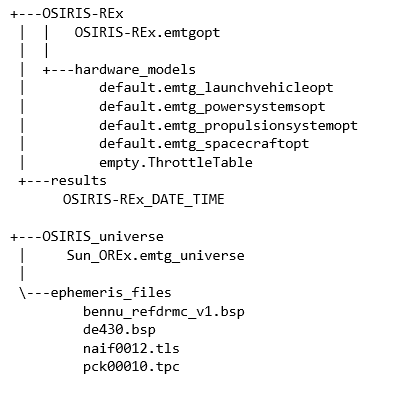
\includegraphics[width=0.6\linewidth]{OSIRIS-REx_folder_structure.png}}
	\caption{\label{fig:folder_structure}Example \ac{EMTG} Mission Directories.}
\end{figure}

\noindent This directory will contain the \ac{EMTG} options file itself, the spacecraft and launch vehicle hardware files in the directory \texttt{hardware\_models}, and the \ac{EMTG} results in the \texttt{results} directory. The other necessary directory is the universe directory containing the \ac{EMTG} Universe file and another directory \texttt{ephemeris\_files} containing all ephemeris files needed for the mission. More information on the Universe directory is provided in the next section and Tutorial 1: OSIRIS-REx. The \texttt{ephemeris\_files} directory name is specific to \ac{EMTG}. If any other name is used, \ac{EMTG} will not be able to find the necessary \ac{SPICE} files.

%%%%%%%%%%%%%%%%%%%%%
\subsection{Universe Directory}
\label{sec:universe_directory}
%%%%%%%%%%%%%%%%%%%%%

Each \ac{EMTG} Journey (Journeys will be explained in detail in the tutorials) uses a \texttt{.emtg\_universe} file listing the relevant bodies (planets, moons, asteroids, etc.) for that mission, which is kept in a directory referenced by the \ac{EMTG} options (.etmgopt) file.

\noindent \ac{EMTG} uses ephemeris files provided by the Jet Propulsion Laboratory Navigation and Ancillary Information Facility (JPL NAIF). The standard ephemeris files for any mission are \texttt{de430.bsp} (planetary ephemeris), \texttt{naif0012.tls} (leap seconds), and \texttt{pck00010.tpc} (frame), although other versions from JPL NAIF may be used. To use a body not in the DE430 ephemeris, include its \texttt{.bsp} file in the \texttt{ephemeris\_files} folder. The \ac{SPICE} ephemeris files can be found on the JPL NAIF site here: \href{https://naif.jpl.nasa.gov/pub/naif/generic_kernels/spk/planets/}{DE files}, \href{https://naif.jpl.nasa.gov/pub/naif/generic_kernels/pck/}{frames}, \href{https://naif.jpl.nasa.gov/pub/naif/generic_kernels/lsk/}{leap seconds}.

\noindent This tutorial series will create two Universe directories and each tutorial will use one or the other.


\end{document}